\documentclass{article}
\usepackage[utf8]{inputenc}
\usepackage{geometry}
\usepackage{graphicx}
\usepackage{pgfplots}
\usepackage{verbatim}
\usepackage{amssymb}
\usepackage{amsmath}
\usepackage{tcolorbox} %needed
\usepackage{comment}
\usepackage{physics}
\tcbuselibrary{listingsutf8}
\newcommand{\ints}{\displaystyle \int \!}
\newcommand{\phix}{\varphi (x)}
\newcommand{\thetax}{\vartheta (x)}
\newcommand{\arctanh}{\text{arctanh}}
\newcommand{\arccoth}{\text{arccoth}}

\geometry{a4paper, left=2cm, right=2cm, top=1cm, bottom=2cm}
\pgfplotsset{compat=1.18}

\begin{document}

$\ints \frac{1}{(x+1)^2(x^2+1)dx}$ \\\\
\textit{De acuerdo al método Integración de Hermite-Ostrogradski.}
\begin{align*}
    \ints \frac{1}{(x+1)^2(x^2+1)}dx &= \frac{\alpha}{x+1} + \ints \frac{\beta}{x+1}dx + \ints \frac{\gamma x + \delta}{x^2+1}dx \\
    \dv{\left(\ints \frac{1}{(x+1)^2(x^2+1)}dx\right)}{x} &= \dv{\left(\frac{\alpha}{x+1} + \ints \frac{\beta}{x+1}dx + \ints \frac{\gamma x + \delta}{x^2+1}dx\right)}{x} \\
    \frac{1}{(x+1)^2(x^2+1)}dx &= \frac{-\alpha}{(x+1)^2} + \frac{\beta}{x+1}dx + \frac{\gamma x + \delta}{x^2+1}dx \\
\end{align*}
\textit{Alinearemos nuestro sistema.}
\begin{align*}
    \Rightarrow
    \quad 1 = -\alpha (x^2+1) + \beta(x+1)(x^2+1) + (\gamma x + \delta)(x^2+2x+1) \\
    1 = -\alpha x^2 - \alpha + \beta x^3 + \beta x^2 + \beta x + \beta + \gamma x^3 + 2\gamma x^2 + \gamma x + \delta x^2 + 2\delta x + \delta
\end{align*}
\textit{i.e. en una matriz...} \\

\begin{table}[h]
\centering
\begin{tabular}{ccccc}
$\alpha$ & $\beta$ & $\gamma$ & $\delta$ & c:G{[}x{]} \\
0                     & 1                    & 1                     & 0                     & 0          \\
-1                    & 1                    & 2                     & 1                     & 0          \\
0                     & 1                    & 1                     & 2                     & 0          \\
-1                    & 1                    & 0                     & 1                     & 1          \\
0                     & 0                    & 0                     & 2                     & 0          \\
0                     & 0                    & 0                     & 1                     & 0          \\
0                     & 2                    & 0                     & 0                     & 1          \\
0                     & 0                    & 2                     & 0                     & 1          \\
0                     & 0                    & 1                     & 0                     & 0          \\
1                     & 1                    & 2                     & 1                     & 0          \\
1                     & 1                    & 0                     & 0                     & 0          \\
1                     & 1                    & 0                     & 1                     & 1         
\end{tabular}
\end{table} 
\textit{Sustituimos nuestros valores de alfa (-0.5), beta (0.5), delta (0) y gamma (0.5).}
\begin{align*}
    \ints \frac{1}{(x+1)^2(x^2+1)}dx &= \frac{\alpha}{x+1} + \ints \frac{\beta}{x+1}dx + \ints \frac{\gamma x + \delta}{x^2+1}dx \\
    &= -\frac{1}{2} \cdot \frac{1}{x+1} + \frac{1}{2} \ints \frac{1}{x+1}dx + \frac{1}{4} \ints \frac{2x}{x^2+1}dx \\
    &= \frac{1}{2} \left[ -\frac{1}{x+1} + ln|x+1| + \frac{1}{2}ln(x^2+1) \right] + c
\end{align*}

\newpage
$\ints \frac{x^5}{\sqrt{1-x^2}}dx$ \\\\
\textit{Haremos el siguiente cambio de variable.} \\
\begin{align*}
\phix &= (1-x^2)^{\frac{-1}{2}} \\
x &= \sqrt{1- \phix^{-2}} \\
dx &= \frac{\phix^{-3}d\phix}{2\sqrt{1-\phix^{-2}}}
\end{align*}
\begin{align*}
    \Therefore \ints \frac{x^5}{\sqrt{1-x^2}}dx &= \ints \sqrt{1- \phix^{-2}}^5 \phix \cdot \frac{\phix^{-3}d\phix}{\sqrt{1-\phix^{-2}}} \\
    &= 2^{-1} \ints (1- \phix^{-2})^2(\phix)(\phix^{-3})d\phix \\
    &= 2^{-1} \ints (1- \phix^{-2})^2 \cdot \phix^{-2} d\phix \\
    &= 2^{-1} \ints (1- 2\phix^{-2} + \phix^{-4}) \cdot \phix^{-2} d\phix \\
    &= 2^{-1} \ints (\phix^{-2} - 2\phix^{-4} + \phix^{-6}) d\phix \\
    &= 2^{-1} [-\phix^{-1} + \frac{2}{3\phix^{3}} - \frac{1}{5\phix^{5}}] + c
\end{align*}
\newpage
$\ints \frac{1}{\sqrt{\tan x}} dx$ \\\\
\textit{Haremos el siguiente cambio de variable.}\\
\begin{align*}
    \phix &=  \sqrt{\tan x} \\
    \arctan (\phix^2) &= x \\
    \frac{2\phix d\phix}{\phix^4 + 1} &= dx
\end{align*}
\begin{align*}
    \ints \frac{1}{\sqrt{\tan x}} dx &=  \ints 2 \left[ \frac{\phix}{\phix} \right] \left[ \frac{1}{\phix^4 + 1} \right] dx \\
    &= \ints \frac{2}{\phix^4 + 1} dx \\
    &= \ints \frac{\phix^2 + 1 - (\phix^2 -1)}{\phix^4 + 1} d\phix \\
    &= \ints \frac{1+\phix^{-2}-(1 - \phix^{-2})}{\phix^2 + \phix^{-2}} d\phix \\
    &= \ints \frac{1+\phix^{-2}}{\phix^2 + \phix^{-2}} - \frac{1 - \phix^{-2}}{\phix^2 + \phix^{-2}} d\phix \\
    &= \ints \frac{1+\phix^{-2}}{\phix^2 + \phix^{-2}} d\phix - \ints \frac{1 - \phix^{-2}}{\phix^2 + \phix^{-2}} d\phix \\
    &= \ints \frac{1+\phix^{-2}}{(\phix - \phix^{-1})^2 + \sqrt{2}^2} d\phix - \ints \frac{1 - \phix^{-2}}{(\phix + \phix^{-1})^2 - \sqrt{2}^2} d\phix \\
    &= \ints \frac{1+\phix^{-2}}{(\phix - \phix^{-1})^2 + \sqrt{2}^2} d\phix + \ints \frac{1 - \phix^{-2}}{\sqrt{2}^2 - (\phix + \phix^{-1})^2} d\phix \\
    &= \frac{1}{\sqrt{2}} \left[ \arctan (\frac{\phix - \phix^{-1}}{\sqrt{2}}) - \arctanh \left( \frac{\phix - \phix^{-1}}{\sqrt{2}} \right) \right] +c \quad \quad \textit{if $|\phix - \phix^{-1}| < 1$ } \\
    &\,\,\, , \ \frac{1}{\sqrt{2}} \left[ \arctan (\frac{\phix - \phix^{-1}}{\sqrt{2}}) - \arccoth \left( \frac{\phix - \phix^{-1}}{\sqrt{2}} \right) \right] +c \quad \quad \textit{if $|\phix - \phix^{-1}| > 1$ } \\
    &= \frac{1}{\sqrt{2}} \left[ \arctan (\frac{\phix - \phix^{-1}}{\sqrt{2}}) - \frac{1}{2}ln \Bigg| \frac{\phix + \phix^{-1} - \sqrt{2}}{\phix + \phix^{-1} + \sqrt{2}} \Bigg| \right] + c \quad \quad \textit{if $|\phix - \phix^{-1}| \in \mathbb{R}$ } \\
    &= \frac{1}{\sqrt{2}} \left[ \arctan (\frac{\sqrt{\tan x} - \sqrt{\cot x}}{\sqrt{2}}) - \frac{1}{2}ln \Bigg| \frac{\sqrt{\tan x} + \sqrt{\cot x} - \sqrt{2}}{\sqrt{\tan x} + \sqrt{\cot x} + \sqrt{2}} \Bigg| \right] + c \quad \textit{if $|\phix - \phix^{-1}| \in \mathbb{R}$ }
\end{align*}
\textit{Se sugiere que se sume la constante 1.1107207345396 a la función.}

\newpage
$\ints \frac{1}{\sqrt{\cos x + 2\sin x + 3}} \, dx$ \\\\
\textit{Demostremos que no es posible su resolución mediante una cantidad finita de funciones elementales.}
\begin{align*}
    \ints \frac{1}{\sqrt{\cos x + 2\sin x + 3}} \, dx &= \ints \frac{1}{\sqrt{a\cos x + b\sin x + k^2}} \, dx
\end{align*}

\newpage
$\ints \sqrt{3-2x-x^2} \, dx$ \\\\
\textit{Empleamos en un futuro la siguiente sustitución trigonométrica.} \\
\begin{figure} [h]
    \centering
    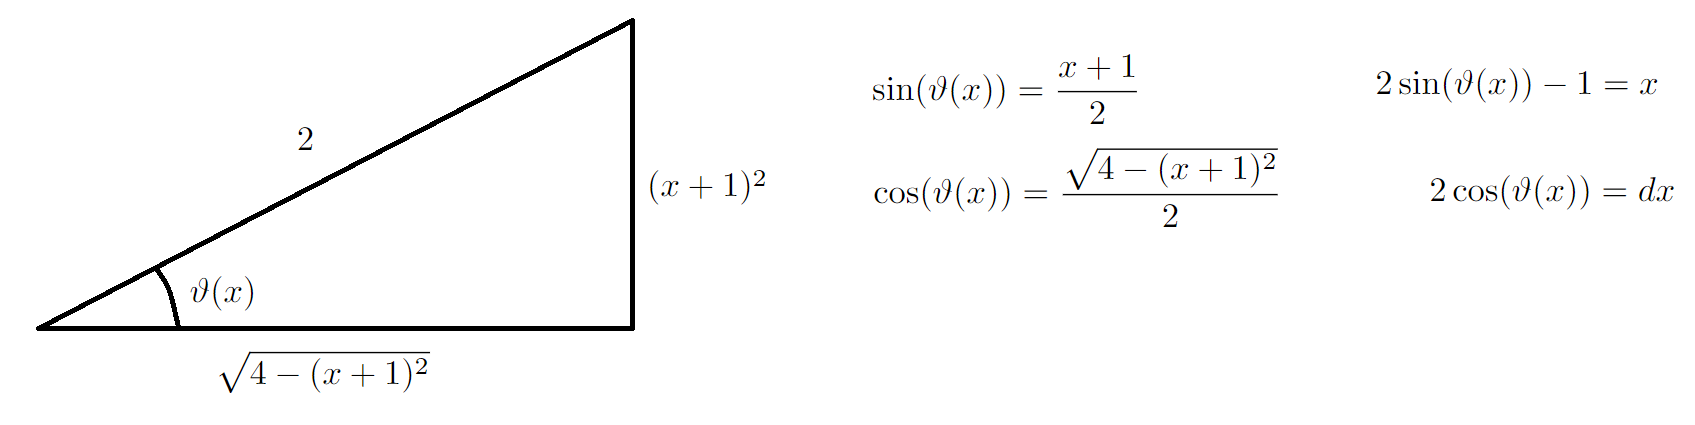
\includegraphics[width=1\linewidth]{Trig.png}
    \label{fig:enter-label}
\end{figure}
\begin{align*}
    \ints \sqrt{3-2x-x^2} \, dx &= \ints \sqrt{4 - (x+1)^2} dx \\
    &= 4 \ints cos^2(\thetax) d\thetax \\
    &= 2\thetax + \sin(2\thetax) + c \\
    &= 2\thetax + 2\sin(\thetax)\cos(\thetax) + c \\
    &= 2\arcsin\left(\frac{x+1}{2}\right) + 2\left( \frac{\sqrt{4-(x+1)^2}}{2} \right)\left( \frac{x+1}{2} \right) + c \\
    &= 2\arcsin\left(\frac{x+1}{2}\right) + \frac{(x+1)\sqrt{3-2x-x^2}}{2} + c
\end{align*}
\newpage
$\ints \frac{1}{(\sin x + \cos x)^2} \, dx$ \\\\
\textit{Consideremos en un futuro una variante en la construcción de la Sustitución Universal (Weierstrass) de primer tipo.}
\begin{figure}[h]
        \centering
        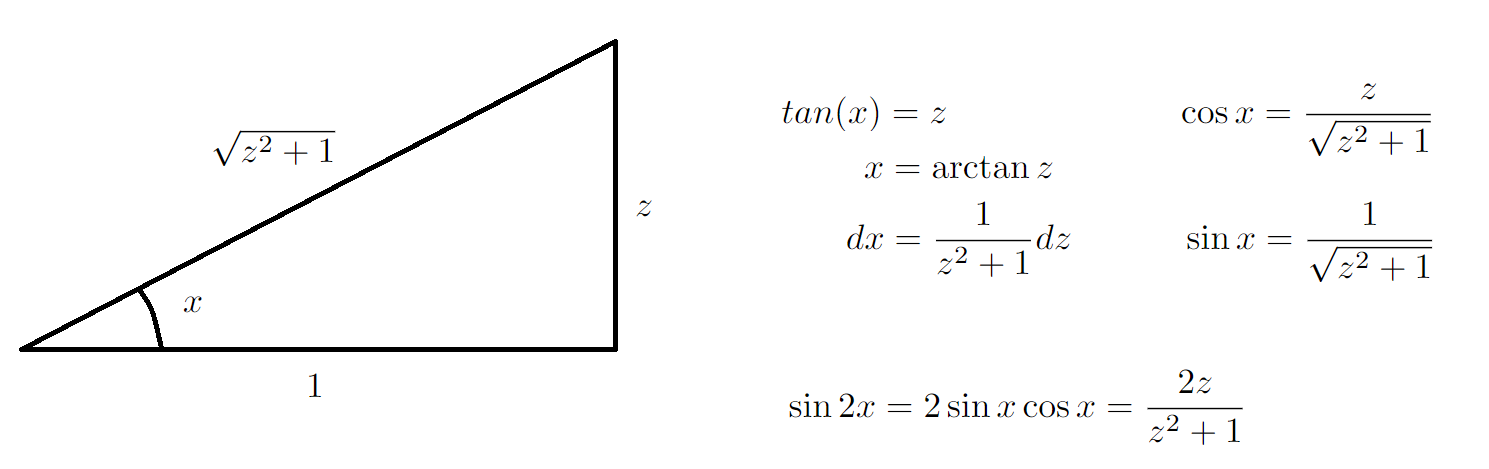
\includegraphics[width=0.8\linewidth]{Universal Sust.png}
        \label{fig:enter-label}
    \end{figure}
\begin{align*}
    \ints \frac{1}{(\sin x + \cos x)^2} \, dx &= \ints \frac{1}{(\cos^2x + \sin^2x) + 2\sin x\cos x}dx \\
    &= \ints \frac{1}{1 + \sin 2x}dx \\
    &= \ints \frac{1}{\frac{z^2+1}{z^2+1} + \sin 2x}dx \\
    &= \ints \frac{1}{\frac{(z^2+1)+2z}{z^2+1}} dx[z] \\
    &= \ints \frac{1}{\frac{(z^2+1)+2z}{z^2+1}} \frac{1}{z^2+1} dz \\
    &= \ints \frac{1}{z^2+1+2z} dz \\
    &= \ints (z+1)^{-2} dz \\
    &= - \frac{1}{z+1} + c \\
    &= - \frac{1}{\tan x+1} + c
\end{align*}
\end{document}